\documentclass[12pt,oneside,spanish]{article}
\usepackage[T1]{fontenc}
\usepackage{times}
\usepackage[utf8]{inputenc}
\usepackage[a4paper]{geometry}
\geometry{verbose,tmargin=2cm,bmargin=2cm,lmargin=3.5cm,rmargin=2cm}
\setcounter{secnumdepth}{3}
\setcounter{tocdepth}{3}
\usepackage{color}
\usepackage[spanish,es-tabla]{babel} % Tabla instead of Cuadro in spanish
\usepackage{amssymb}
\usepackage{amsmath}
\usepackage{psfrag}
\usepackage{multirow}
\usepackage{graphicx}
\usepackage{subfigure}
\usepackage{longtable}
\usepackage{dcolumn}
\usepackage{booktabs}
\usepackage{listings}
\usepackage[unicode=true,linkbordercolor={1 1 1}]{hyperref}

% References styles fo bibtex
\usepackage[square,numbers]{natbib}
\bibliographystyle{abbrvnat}

% Chapter
\usepackage{titlesec}
%\titleformat{\chapter}[block]{\bfseries\scshape\Huge}{}{0pt}{\filcenter}[]
\titleformat{\chapter}[block]{\bfseries\Huge}{}{0pt}{\filcenter}[]

% Heading
\usepackage{fancyhdr}
\pagestyle{fancy}
%\renewcommand{\chaptermark}[1]{\markboth{#1}{}}
%\renewcommand{\sectionmark}[1]{\markright{--- #1}}
\fancyhf{}   %apaga tudo
\fancyhead[C]{\scriptsize\scshape\nouppercase{\leftmark}}
\fancyhead[R]{\oldstylenums\thepage}
\renewcommand\headrulewidth{0pt}
\fancypagestyle{plain}{
	\fancyhead[R]{\bfseries{\oldstylenums\thepage}}
	\fancyhead[C]{}}

% Turn table
\usepackage{fancybox}

% Title page
\title{ 
	
\includegraphics[width=0.35\textwidth]{unsa.eps}\\
	\vspace{0.1cm}
{\large Escuela Profesional de Ingeniería Electrónica \\
\vspace{2cm}
{\small Guía de Laboratorio de Tecnología de la Ingeniería Aeronáutica y Espacial}} \\ 
\vspace{0.1pt} 
\hrulefill \vspace{40pt} \\ 
\textbf{Lab 02: Dinámica de Sistemas Aeroespaciales}\\ 
\vspace{30pt} \hrulefill}
\author{\scshape{\textbf{ }}
\vspace{30pt} \\
	\vspace{0.5cm}
	{\small Alumnos}\\
	{\Large Dolmos Becerra, Uriel Frankdali}\\
	{\Large Pocohuanca Fernandez, Jeremin}\\
	{\Large Torres Cori, Josue Breithner}\\
	\vspace{3cm}\\
{\small Profesor: Dr. Juan C. Cutipa Luque}\\
\vspace{20pt}
}
\date{11 de junio de 2021}

\begin{document}

\pagenumbering{gobble}

\maketitle

\newpage

\begin{abstract}
Este documento constituye la guía de laboratorio que deberá ser completada por los alumnos integrantes durante las horas de laboratorio de la asignatura de Tecnología de la Ingeniería Aeronáutica y Espacial.

\end{abstract}


\pagebreak

\tableofcontents
%\listoffigures
%\listoftables

\newpage
\pagenumbering{arabic}

%  ---------------------- here goes your report -------------
%
\section{Objetivo}
Entender la dinámica de los cuerpos rígidos y las tecnologías usadas en la ingeniería aeroespacial.
\section{Fundamento Teórico}
En esta parte, el alumno recolecta la información necesaria para realización de su experiencia. La fuente principal de información es el contenido de la unidad 2 según sílabo de la asignatura de Tecnología de la Ingeniería Aeronáutica y Espacial.

\section{Materiales y Equipamientos}
\begin{itemize}
    \item Computador Laptop.
    \item Gnu-Octave\footnote{Software libre que se distribuye bajo la licencia GPL ver 3, disponible en \url{https://www.gnu.org/software/octave/}}.
    \item Python 2 y Python 3\footnote{Este lenguaje de programación es uso libre y está disponible en \url{www.python.org}}.
    \item Cocalc, plataforma basada en web para desarrollo de algoritmos en la nube (disponible en \url{https://cocalc.com}).
\end{itemize}

\section{Procedimientos}
Los procedimientos de la presente experiencia de Laboratorio son:
\begin{enumerate}
\item Abrir su cuenta Cocalc, y crear un proyecto de nombre 'Lab 02 TIAE 2021 A'. Ingrese al proyecto creado y cree un nuevo archivo de nombre 'vanderpol.py'.
\begin{lstlisting}[language=Python,numbers=left,numbersep=5pt,numberstyle=\tiny, frame=single, basicstyle=\footnotesize]
import numpy as np
from scipy import integrate
import matplotlib.pyplot as plt

# define la funcion o dinamica de vanderpol
def vdp1(t, y):
    return np.array([y[1], (1 - y[0]**2)*y[1] - y[0]])
    
ti, tf = 0, 20                 # tiempo de inicio y fin de solucion
t = np.linspace(ti, tf, 100)   # el vector tiempo t con 100 pasos
y0 = [2, 0]                    # condiciones inicial
y = np.zeros((len(t), len(y0)))   # define el arreglo de la solucion
y[0, :] = y0
r = integrate.ode(vdp1).set_integrator("dopri5")  # integracion
                                                  # numerica
r.set_initial_value(y0, ti)    # configura las condiciones iniciales
for i in range(1, t.size):
   y[i, :] = r.integrate(t[i]) # conseguir mas valores,
                               # completa el arreglo
   if not r.successful():
       raise RuntimeError("no se consigue integrar")
plt.plot(t, y)
plt.show()
\end{lstlisting}

\begin{figure}[h]
    \centering
    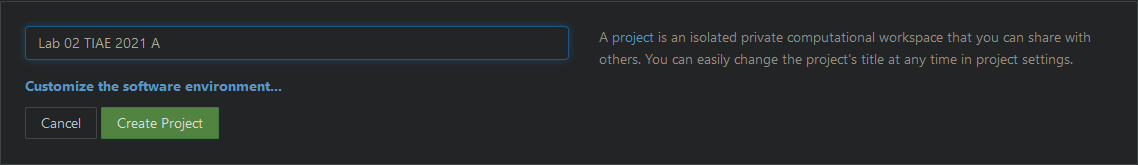
\includegraphics[scale=0.5]{Cocalc/CreacionProyecto.png}
    \caption{Creación del proyecto}
    \label{fig:my_label1}
\end{figure}
\begin{figure}[h]
    \centering
    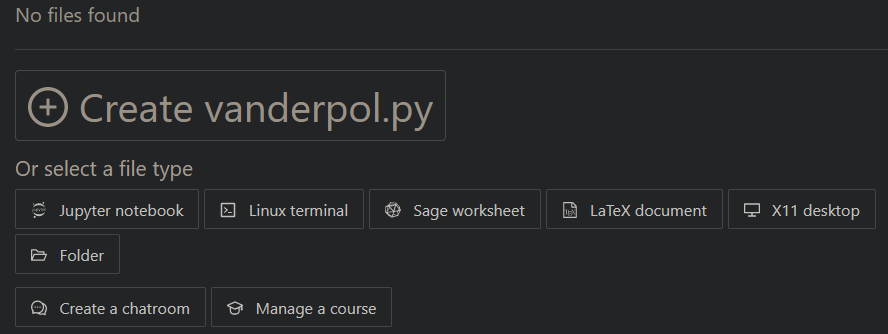
\includegraphics[scale=0.5]{Cocalc/CrearVanderpol.png}
    \caption{Creación de archivo Vanderpol.py}
    \label{fig:my_label2}
\end{figure}
\item En el mismo proyecto, crear un archivo de nombre 'myDesktop.x11'. En el terminal, localizado al lado izquierdo de la pantalla digitar 'gedit vander.py', deberá aparecer una ventana de editor de texto al lado derecho, en donde debe introducir el código anterior (ver Fig. \ref{fig:vander}). Grabe el contenido del editor derecho (botón 'save'), cierre la ventana.
\begin{figure}[h]
    \centering
    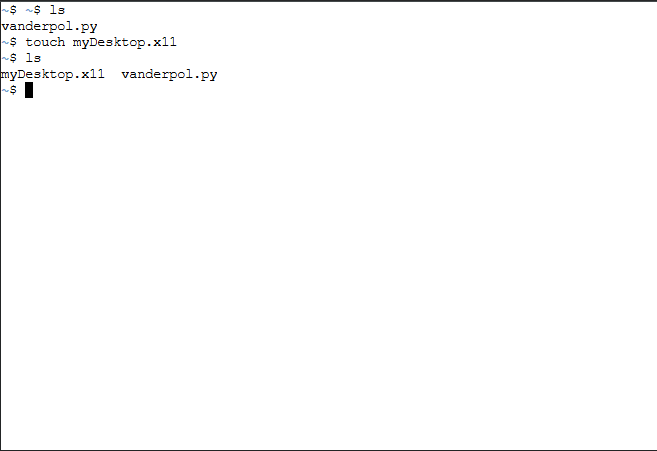
\includegraphics[scale=0.7]{Cocalc/CrearDesktop.png}
    \caption{Creación de archivo myDesktop.x11}
    \label{fig:my_label}
\end{figure}
\newpage
\begin{figure}[h]
    \centering
    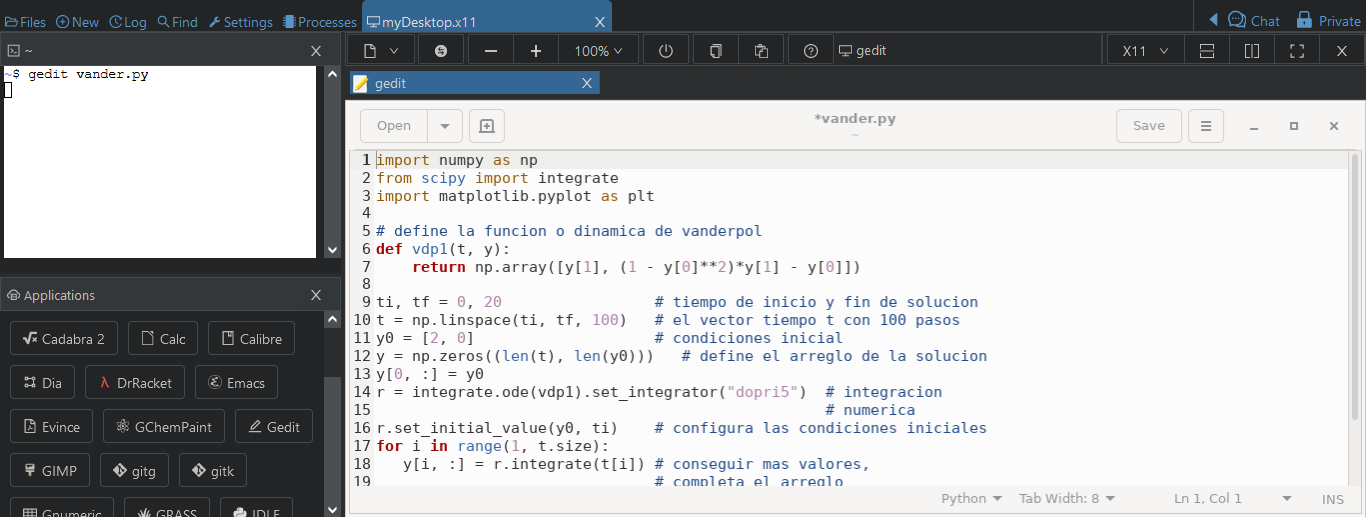
\includegraphics[scale=0.4]{Cocalc/Editarvander.png}
    \caption{Escribir codigo python con el programa grafico Gedit en vander.py}
    \label{fig:my_label}
\end{figure}
\item En la ventana de terminal (lado izquierdo) ejecutar el archivo 'vander.py' con la instrucción 'python3 vander.py' y obtener la solución numérica de la Fig. \ref{fig:vanderResult}.
\begin{figure}[h]
    \centering
    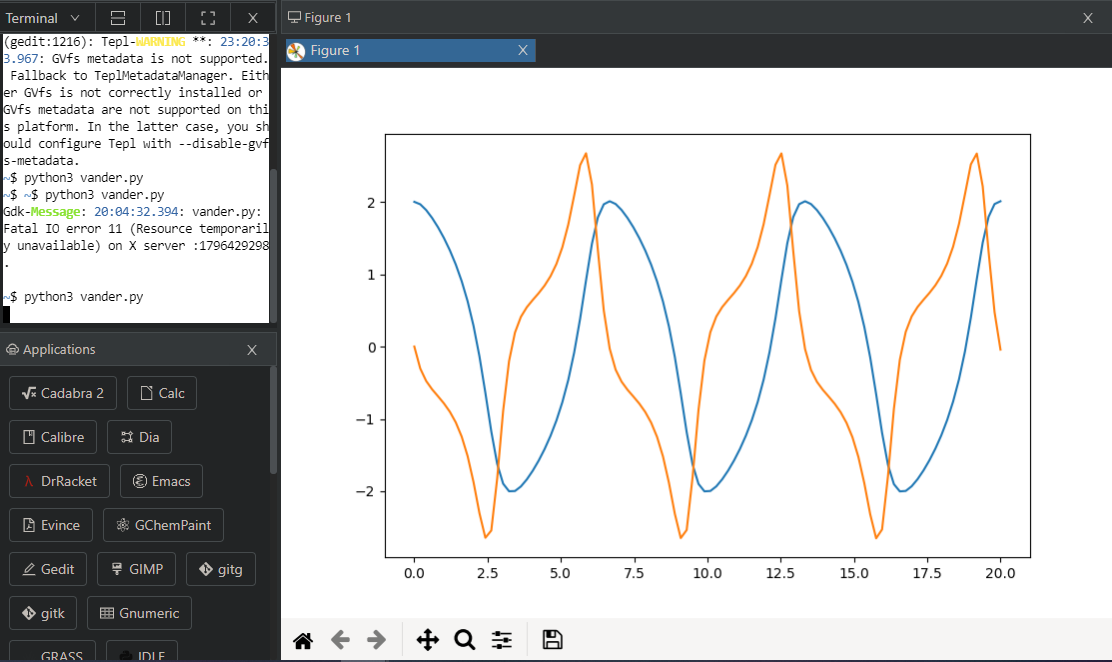
\includegraphics[scale=0.5]{Cocalc/VanderGrafico.png}
    \caption{Resultado de archivo 'Vander.py'}
    \label{fig:my_label}
\end{figure}
\item La dinámica del 'helicóptero' ingenuity recientemente enviado a Marte en el proyecto 'perseverance' se presenta en artículos publicados por la NASA \footnote{\url{https://rotorcraft.arc.nasa.gov/Publications/files/ERF2017_final.pdf} y \url{https://rotorcraft.arc.nasa.gov/Publications/files/Balaram_AIAA2018_0023.pdf}}. Identifique las ecuaciones de cuerpo rígido.

%\begin{figure}[h]
%    \centering
%    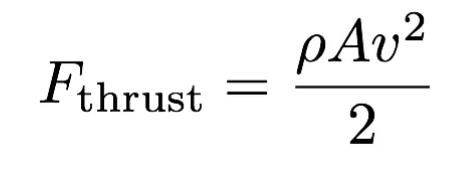
\includegraphics[width=5cm]{Ecuaciones\img1.png}
%\end{figure}
\begin{equation*}
    F_{thrust}=\frac{\rho A v^2}{2}
\end{equation*}
%\begin{figure}[h]
%    \centering
%    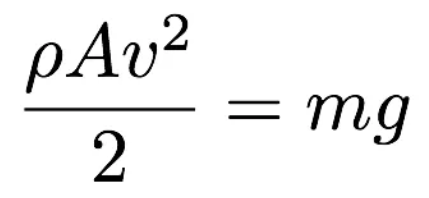
\includegraphics[width=5cm]{Ecuaciones\img2.png}
%\end{figure}
\begin{equation*}
    \frac{\rho A v^2}{2}=mg
\end{equation*}
%\begin{figure}[h]
%    \centering
%    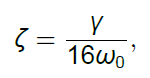
\includegraphics[width=5cm]{Ecuaciones\img3.png}
%\end{figure}
\begin{equation*}
    \zeta=\frac{Y}{16 \omega_{0}}
\end{equation*}
%\begin{figure}[h]
%    \centering
%    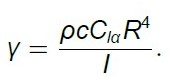
\includegraphics[width=5cm]{Ecuaciones\img4.jpg}
%\end{figure}
\begin{equation*}
    Y=\frac{\rho cC_{l\alpha}R^4}{I}
\end{equation*}
\item De los mismos artículos, indique la relación entre inercia aparente.
%\begin{figure}[h]
%    \centering
%    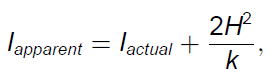
\includegraphics[width=5cm]{Ecuaciones\img5.png}
%\end{figure}
\begin{equation*}
    I_{aparente}=I_{actual}+\frac{2H^2}{k}
\end{equation*}
%\begin{figure}[h]
%    \centering
%    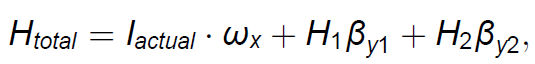
\includegraphics[width=5cm]{Ecuaciones\img6.png}
%\end{figure}
\begin{equation*}
    H_{Total}=I_{actual}. \omega_{x}+H_{1}\beta_{y1}+H_{2}\beta_{y2}
\end{equation*}
%\begin{figure}[h]
%    \centering
%    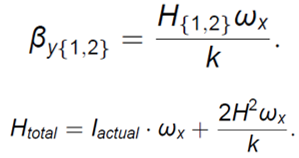
\includegraphics[width=5cm]{Ecuaciones\img7.png}
%\end{figure}
\begin{equation*}
    \beta_{y\left\lbrace1,2\right\rbrace}=\frac{H_{\left\lbrace1,2\right\rbrace}\omega_{x}}{k}
\end{equation*}
\begin{equation*}
    H_{Total}=I_{actual}. \omega_{x}+\frac{2 H^2 \omega_{x}}{k}
\end{equation*}
\item Basado en la solución numérica presentada anteriormente, implemente la dinámica de un vehículo aeroespacial (avión, cuadrirotor, avión, satélite, submarino, etc).

La fórmula se puede utilizar para aproximar el efecto para un helicóptero con palas discretas, reemplazando Iactual con la inercia media, y k con la constante de resorte de cada hoja, multiplicado por N/2, donde N es el número de hojas en cada rotor. Aplicado al ejemplo de la última sección,
obtener Iaparente = 0.029 kg m2, que es consistente con el respuesta observada

\end{enumerate}helicóptero’ ingenuity recientemente enviado a Marte en el proyec-to ’perseverance’ s

\textbf{Recomendación:} Debe incluir al profesor (jccluque@gmail.com) como colaborador de su proyecto en Cocalc.
\section{Cuestionario}
\begin{enumerate}
    \item Como varían las dinámicas de cuerpo rígido cuando la coordenada del eje 'z' apunta fuera del centro de la tierra.\\
Varían de forma opuesta, quiere decir que el movimiento de desplazamiento sera contrario a lo indicado si el sentido de giro se mantiene.
    
    \item Indique la diferencia entre esfuerzos internos y esfuerzos externos en el fuselaje de una aeronave comercial.\\ \\
    El fuselaje es el cuerpo estructural de la aeronave, que
aloja a los pasajeros o carga y combustible, junto con los sistemas y equipos. Se considera la parte central por que a ella se acoplan directamente o indirectamente el resto de los componentes como las superficies aerodinámicas, el tren de aterrizaje y el grupo motopropulsor. En aeronaves monomotor el fuselaje contiene al grupo motopropulsor y a la cabina de la tripulación; sirve también de soporte a las alas y estabilizadores; y lleva el tren de aterrizaje.\\
Un avión comercial buscará un promedio entre volumen
para carga y pasajeros a la sección recta del fuselaje tenderá a ser circular para aliviar las cargas de presurización de la cabina, ya que de esta forma los esfuerzos generados son uniformes.\\
Los tres esfuerzos básicos son la tracción, compresión y esfuerzos cortantes. Y sus combinaciones son: flexión, torsión y esfuerzos de contacto.
\begin{itemize}
    \item Efecto de Flexión en la alas
    \item Efectos de Flexión y Torsión en el fuselaje
    \item Efecto de Flexión en el fuselaje
\end{itemize}


    \item Explique las ecuaciones de momentum angular usando el principio de funcionamiento de una bicicleta.\\
   se suspende la rueda de bici con ayuda de una cuerda atada a un extremo del eje. Mientras se sujeta el otro extremo se hace girar la rueda y después se suelta ese extremo. La rueda no cae, sino que comienza a girar en el plano horizontal. Para explicarlo hay que recordar la relación entre el torque neto $ \vec{\tau} $ que se ejerce sobre un cuerpo que gira con momento angular $ \vec{L}$\\
   $\vec{\tau} = \frac{d(\vec{L})}{dt} $\\
   En nuestro caso, el torque se produce por el peso de la rueda a una distancia݈ del punto de sujeción de la cuerda. Al tener este torque una dirección perpendicular al momento angular de giro de la rueda, su efecto va a ser el de cambiar la dirección del momento angular (no su módulo), lo que lo hace girar en el plano horizontal. Se puede estimar la velocidad angular de
precesión $ \omega $ si se conoce el momento angular inicial de giro de la rueda $ \vec{L} $ ya que $ \theta = \mid (\frac{d(\vec{L})}{dt}) \mid $ con $ \theta$ ángulo de giro del eje de la rueda en el plano horizontal. Por lo que  $ \omega = \frac{d(\theta)}{dt}=\frac{\mid \tau \mid}{\mid \vec{L} \mid } = \frac{Mgl}{\mid \vec{L} \mid } $, con ܯ masa de la rueda, ݃
aceleración de la gravedad y ݈ distancia del punto de sujeción de la cuerda al
centro de masas de la rueda. 

    
\end{enumerate}
\textbf{Obs.} Cuando no hay interrogantes, se recomienda discutir los resultados obtenidos durante el procedimiento de la experiencia.

\begin{figure}
    \centering
    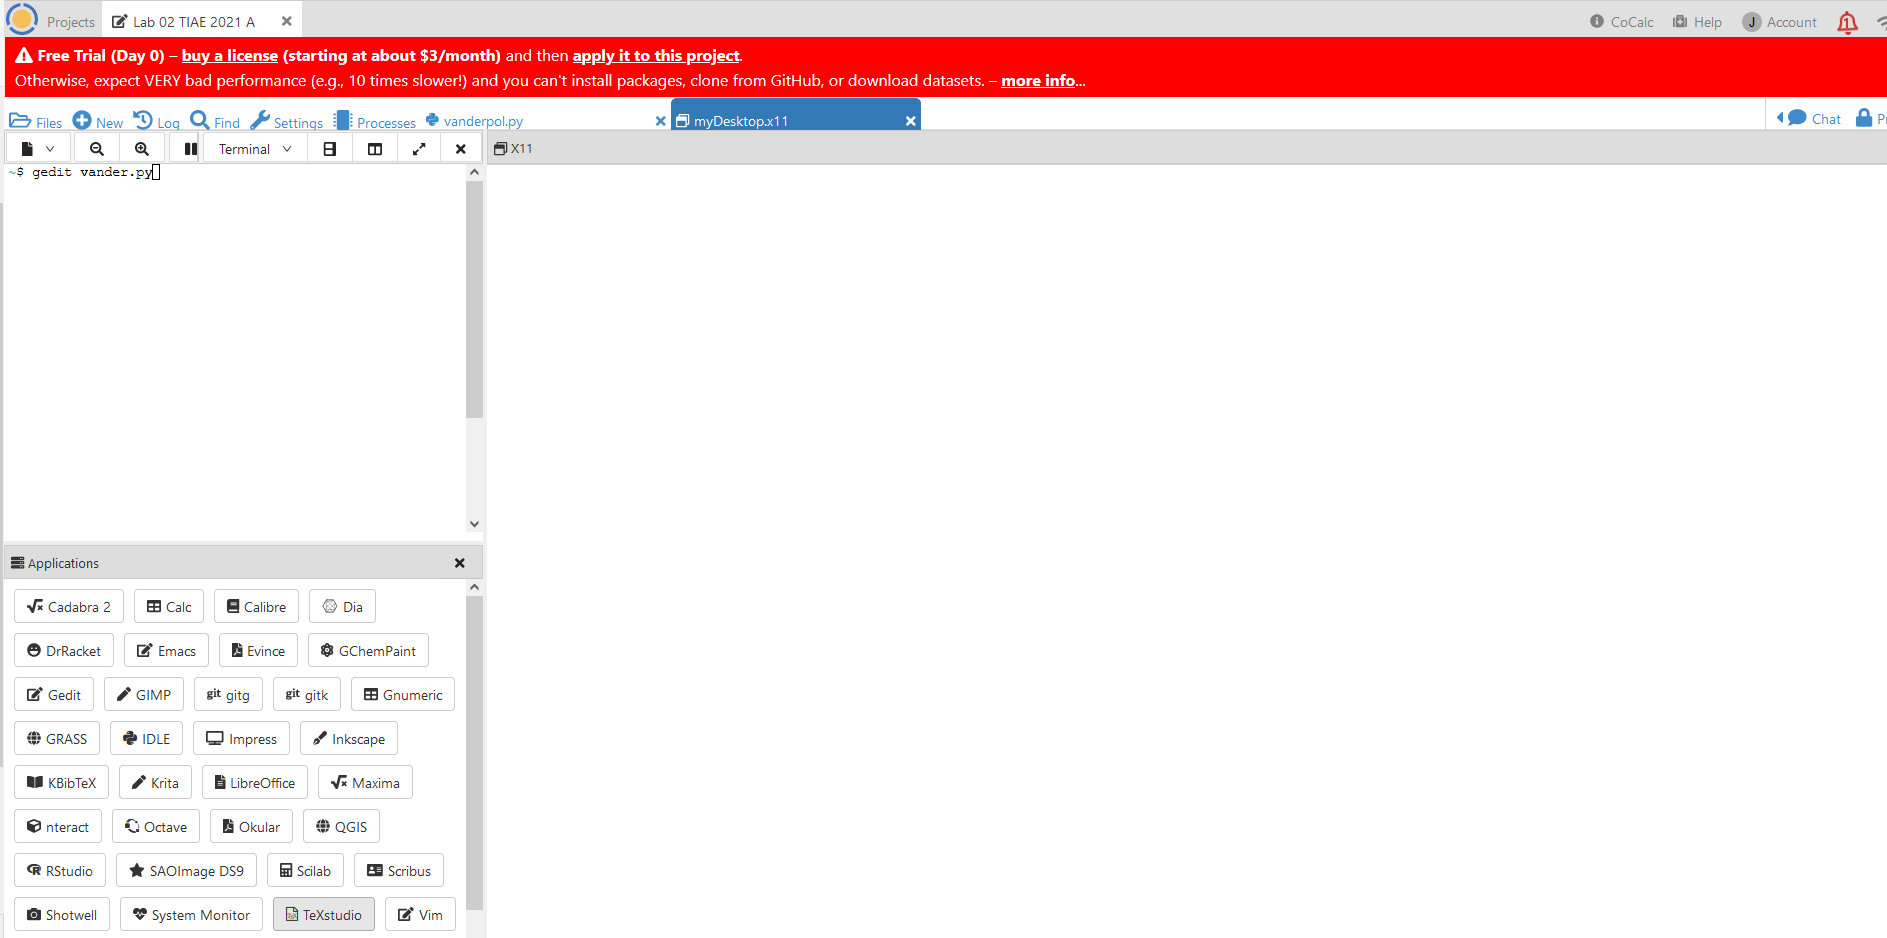
\includegraphics[width=12cm]{vander.png}
    \caption{Proyecto 'vander.py' dentro de 'mydesktop.x11'.}
    \label{fig:vander}
\end{figure}

\begin{figure}
    \centering
    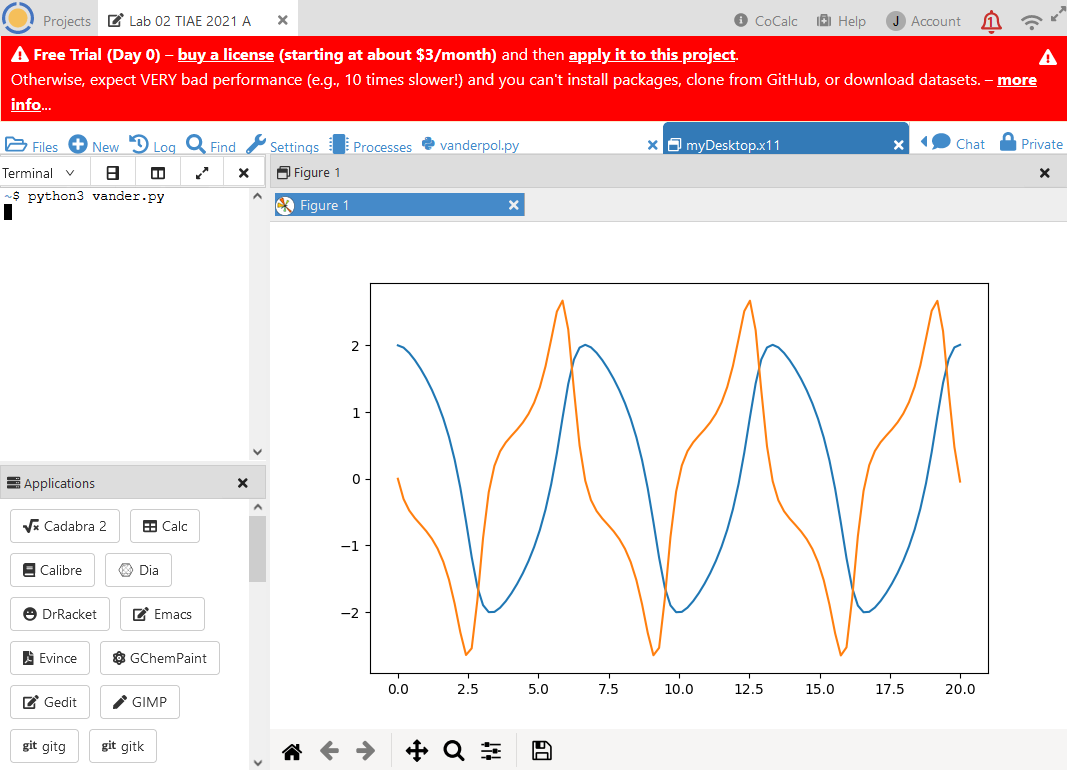
\includegraphics[width=12cm]{vanderResult.png}
    \caption{Resultado de la simulación 'vanderResult.py'.}
    \label{fig:vanderResult}
\end{figure}

\section{Conclusiones}
Aquí debe concluir de forma sucinta sobre la experiencia realizada y colocar observaciones que considere pertinentes.
Puede encontrar más información en las referencias del silabo del curso o en el texto de \cite{Triantafyllou:2002,fossen:2011}.
\begin{itemize}
    \item Las ecuaciones de dinámica de cuerpo rígido desarrolladas en la tierra son referencia para el helicóptero ingenuity a marte, considerando la diferencia de gravedad y densidad atmosférica del planeta rojo.
\end{itemize}
\section{Repositorio}
\begin{itemize}
    \item Github: 
    \url{https://github.com/jtorrescor/Lab-02-TIAE-2021-A}.
    \item Latex: 
    \url{https://www.overleaf.com/2161555411cjpfyttxkdzp}.
\end{itemize}
\newpage
%\fancyhead[C]{\scriptsize\scshape\nouppercase{\leftmark}}
\addcontentsline{toc}{section}{Referencias Bibliográficas} %
%
\bibliography{referencias}
\appendix

\newpage
\addcontentsline{toc}{section}{Apéndice} %
\section*{Apéndice}

\newpage
\addcontentsline{toc}{section}{Rúbrica} %
\section*{Rúbrica}
\begin{itemize}
\item[e1:] Identifica y diagnostica problemas y los prioriza de acuerdo a su impacto o relevancia.
\item[e2:] Formula soluciones coherentes y realizables usando normas y estándares apropiados.
\item[e3:] Utiliza las técnicas y metodologías de la ingeniería electrónica para plantear, analizar y resolver problemas de ingeniería.
\item[e4:] Maneja equipos e instrumentos y utiliza software especializado propio del ejercicio profesional.
\end{itemize}
La tabla \ref{tab:rubricas} refleja la evaluación del estudiante respecto este informe y mediante entrevistas. 

\begin{table}[h!]
\caption{Rúbrica según Resultados del Estudiante}
\centering
\begin{tabular}{lcccc}
\hline 
Alumno & e1 & e2 & e3 & e4\tabularnewline
\hline 
\hline 
Dolmos Becerra, Uriel Frankdali &  &  &  & \tabularnewline
\hline 
Pocohuanca Fernandez, Jeremin &  &  &  & \tabularnewline
\hline 
Torres Cori, Josue Breithner &  &  &  & \tabularnewline
\hline
\end{tabular}
\label{tab:rubricas}
\end{table}
\end{document}
